\documentclass[a4paper]{report}

\usepackage{graphicx}
\usepackage[english]{babel}
\usepackage[utf8]{inputenc}
\usepackage[T1]{fontenc}
\usepackage{ragged2e}
\usepackage{hyphenat}
\usepackage{lmodern}
\usepackage{fancyhdr}
\usepackage[toc,page]{appendix}
\usepackage{tabularx}
\usepackage{float}
\usepackage{amsmath}
\usepackage{indentfirst}

\begin{document}
    \centering
    \LARGE{\textsc{VIETNAM AVIATION ACADEMY}}\\
    \vspace{3mm}
    \normalsize{Department of Telecommunication - Electronics Engineering Technology} \\
    \vspace{3mm}
    \large{LOCATION IN HO CHI MINH CITY} \\
    \vspace{3mm}
    
\includegraphics[scale=0.3]{logo.jpg} \\
    \vspace{3mm}
    \normalsize{PROJECT REPORT: } \\ 
    \vspace{15mm}
    \huge{\textbf{"NDB radar detector module using Arduino"}} \\
    \vspace{20mm}
    \normalsize{Written by} \\
    \vspace{3mm}
    \large{\textbf{\textit{Nguyen Van Anh Tuan}}} \\
    \vspace{3mm}
    \textbf{{\large{\textit{Roll.No.1753020018}}}} \\
    \vspace{15mm}
    \large{Under the guidance of} \\ 
    \vspace{10mm}
    \centerline{\textbf{\large{Cao Xuan Kim Anh}}}
    
    %Lines down here is set header and footer
    \pagestyle{fancy}
    \fancyhf{}
    \rhead{Radar detector module}
    \lhead{Anh Tuan}
    \cfoot{\today}
    \renewcommand{\headrulewidth}{2pt}
    \renewcommand{\footrulewidth}{1pt}

    % \setlength\parindent{24pt} is indentation.
    \newpage
    \centering
    \centerline{\textbf{\huge{PREAMBLE}}}
    \vspace{10mm}
    \begin{flushleft}
        In VietNam's aviation industry today as well as in the world, radar is along-range object 
        detection system that uses radio waves to etablish certain parameters of an object like 
        its range, speed and position. Radar technology is used in aircrafts, missiles, marinem, 
        weather predictions and automobiles. Even though the title says "Arduino Radar 
        Project" technically the projects is based on Sonar technology as i will be using 
        an Ultrasonic Sensor to determine the presence of any object in particular range.
    \end{flushleft}
    \begin{flushright}
        \textbf{Auth. Nguyen Van Anh Tuan}
    \end{flushright}
    \thispagestyle{plain}

    \newpage
    \tableofcontents

    \chapter{Introduction}
    \thispagestyle{fancy}
    \fancyhf{}
    \fancyhead[L]{Anh Tuan}
    \fancyhead[R]{Radar detector module}
    \raggedright
    \fancyfoot[R]{Page \thepage}
    \section{PRELIMINARY INTRODUCTION}
    \subsection{The reason why to choose project}
        With the passion for aviation as well as passion for technology and equipment realted to 
        it, i decided to choose an aviation-related project in this project. Fortunately, my project 
        this time is on topic of embedded programming. So, i choose project named "NDB radar 
        detector module using Arduino". In this project, i will rely 
        on the NDB radar to make a small scale NDB radar detector model. So, to get 
        started in this project, we need to know what NDB radar is and how it works. \\
    \vspace{5mm}
        Recognize the continuous development of aviation technology. I want to add my own 
        knowledge about how a radar system works and a bit of creative idea for this device 
        that came along during i make this project. And that's why i choose this project for myself. \\
    \vspace{5mm}
    \textbf{Block diagram}
    \begin{figure}[ht]
        \centering
        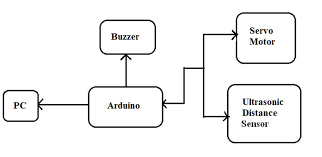
\includegraphics[scale=0.7]{block_diagram.png}
        \caption{\label{fig:pic}Block diagram for radar model}
    \end{figure}
    \linebreak
    \par You may ask how the processing application works here. It's very simple, the 
    Ultrasonic sensor collects the object information with the help of Arduino and passes 
    it to processing application, there is a simple Graphics application implemented which 
    mimic a radar screen.
    \subsection{Target Research}
        The short term goal of this topic is with the desire to learn and supplement the 
        knowledge that in the course of research. With the long term goal, i want to perform 
        the topic in the best way i can. As well as improve the errors of myselft. And also, 
        i want to additional the knowledge i haven't learned at my school.
    \subsection{Object and position research}
    \vspace{3mm}
        \begin{itemize}
            \item \textbf{Object Research:} The object that i study is the sensor system 
        installed on the air traffic control station or installed on robots that detect 
        objects and avoid them.
            \item \textbf{Position Research:} My reserach is based on the application of radar 
        to detect missing vehicles or to apply air traffic control as call as "Primary Surveillance Radar".
        \end{itemize} 
    \subsection{Method of research}
        \begin{itemize}
            \item \textbf{Observation Method:} By observing directly at air traffic control 
        and also via movies or aviation videos on internet.
            \item \textbf{Method of analysis:} Looking for some similar projects that have 
        been made available online, from the detailed data of those projects, i draw some 
        methods and experience for my project. Avoid mistakes in my project.
        \end{itemize}
    \subsection{Structure Project}
        My article is divided into three main sessions, summarized as follow: 
        \begin{itemize}
            \item In the first chapter, i will focus on brief introduce my project, presenting 
        some of the research content on the topic of the method of conducting research that 
        gives practical results during the project research process.
            \item The second chapter, is an introduction about some of basic project implementation 
        theories, to present related project i'm working on it.
            \item Chapter three is the chapter where i introduce the main content of my project, 
        presenting a basic article of project and how it works, accompany it with some examples.
            \item The next chapter is the construction and circuit design on Kicad Altium software 
        and the implementation of hardware construction.
            \item And the final chapter is the final section where i draw some conclusion during 
        project implementation, as well as point out my own strengths weaknesses in the course of my project.
        \end{itemize}
    \section{BASIC THEORY}
    \subsection{Some research related to the project}
        
\end{document}